\documentclass{article}

\usepackage{Paper}
\renewcommand\theadfont{\bfseries}
\setcellgapes{2pt}

\fancyhead[L]{Group 4}

\geometry{
    a4paper,
    total={170mm, 257mm},   
    left=20mm,
    top=20mm,
    bottom=15mm
}

\pdftitle{Group4-Synchronous-Generator}

% === TEXT ===
\begin{document}
\thispagestyle{empty}

\begin{minipage}{0.7\textwidth}
    \vspace*{-.8cm} \hspace*{-0.3cm}
    
\includegraphics[width=.5\textwidth]{media/hslu-logo.png}
\end{minipage}

\vspace*{1.5cm}

\textbf{\huge Lab report}\\[.75cm]
\begin{center}
    \textbf{\huge EUG -- Grid synchronisation and}
    
    \textbf{\huge automatic generator control}\\[0.8cm]
    
    
\includegraphics[\lw=.8]{media/E1S2a/picture3.png}\\
\end{center}

\vfill

\textbf{\Large Electric Power Grids}\\[.5cm]
{\large
\textbf{Group 4}\\[1ex]
Bürli Norman\\[1ex]
Frongillo Matteo\\[1ex]
Monti Antonio\\[1ex]
Moos Michael}
\vfill

\newpage
\tableofcontents
\thispagestyle{fancy}
\pagebreak
\section{Grid synchronisation and automatic generator control course}
Synchronisation of a synchronous generator with the electrical grid requires equal
voltage magnitude, frequency, phase sequence and phase angle between generator and grid.
If these conditions are not fulfilled, large transient currents and mechanical stresses
may occur during connection.

\subsection{Manual synchronisation with the aid of a dark lamp circuit}
In this experiment, synchronisation was performed manually using the dark
lamp method and a synchronoscope. For manual synchronisation of a synchronous generator
to the power grid, the dark lamp synchronisation method was used.
The lamps were connected between identical phases of the generator
and the grid, as shown in \autoref{fig:darklamp}.
\begin{figure}[H]
    \centering
    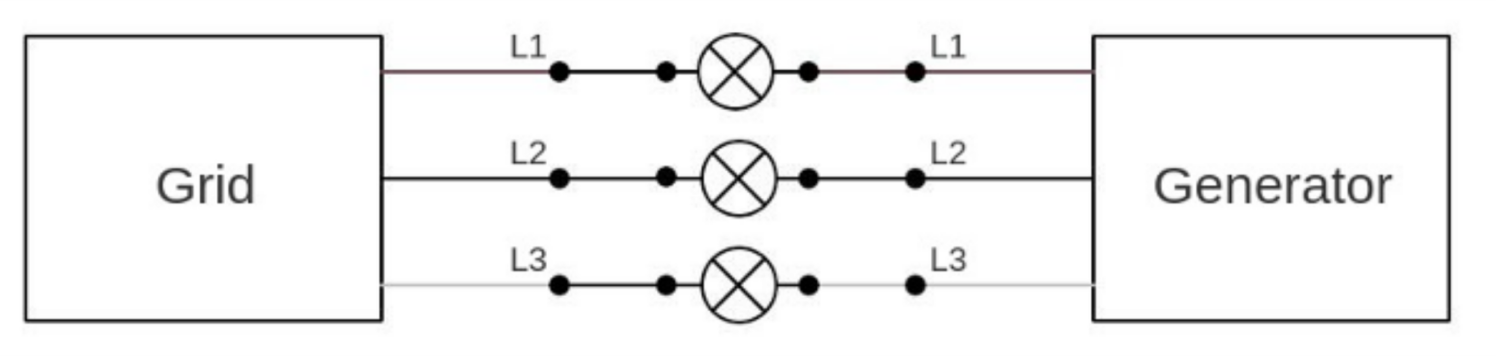
\includegraphics[\lw=.6]{media/E1S1/darklamp.png}
    \caption{Dark lamp circuit}
    \label{fig:darklamp}
\end{figure}

If the voltages of the generator and the grid were in opposite phase, all three lamps
lit up brightly due to the high voltage difference. As the generator voltage approached
the grid voltage in magnitude and phase angle, the voltage difference decreased and the
lamps became darker. Synchronisation was achieved when the lamps were nearly dark,
indicating that the phase voltages were closely matched. At this moment, the generator
could be connected safely to the grid.

In addition to the lamp circuit, the experimental setup included a dual-range voltmeter,
a synchronoscope, a zero-voltmeter and a dual-range frequency meter. The voltmeter was
used to compare the generator and grid voltages. The synchronoscope indicated the phase
angle difference and the frequency difference between the generator and the grid. For
synchronisation, the green LED SYNC must be alight. The zero-voltmeter measured the
voltage difference between corresponding phases, which approached 0 V during
synchronisation. The frequency meter displayed the frequencies of both systems, which
had to match before connection.

\begin{figure}[H]
    \centering
    \includegraphics[\lw=.8]{media/E1S1/picture2.png}
    \caption{Experimental setup}
    \label{fig:exp-setup}
\end{figure}

\newpage
\autoref{fig:exp-setup} shows the experimental setup used during the laboratory session.
The generator was initially operated slightly above synchronous speed (+2 rpm). The
excitation voltage was then adjusted until the generator voltage matched the grid
voltage. Afterwards, the generator speed was reduced slowly until the synchronoscope
rotated slowly and the phase angle approached synchronism. Once the synchronoscope
indicated synchronous operation and the lamps became dark, the generator was connected
to the grid using the synchronisation switch.

\autoref{fig:meter} shows the measurement instruments and synchronoscope during the
synchronisation process. On the top left, the dual-range voltmeter shows twice 400 V, the
zero voltmeter below shows 0 volts. On the right side, the dual-range frequency meter
shows both systems to be at 50 Hz, and below, the synchronoscope has the green SYNC LED
alight.

\begin{figure}[H]
    \centering
    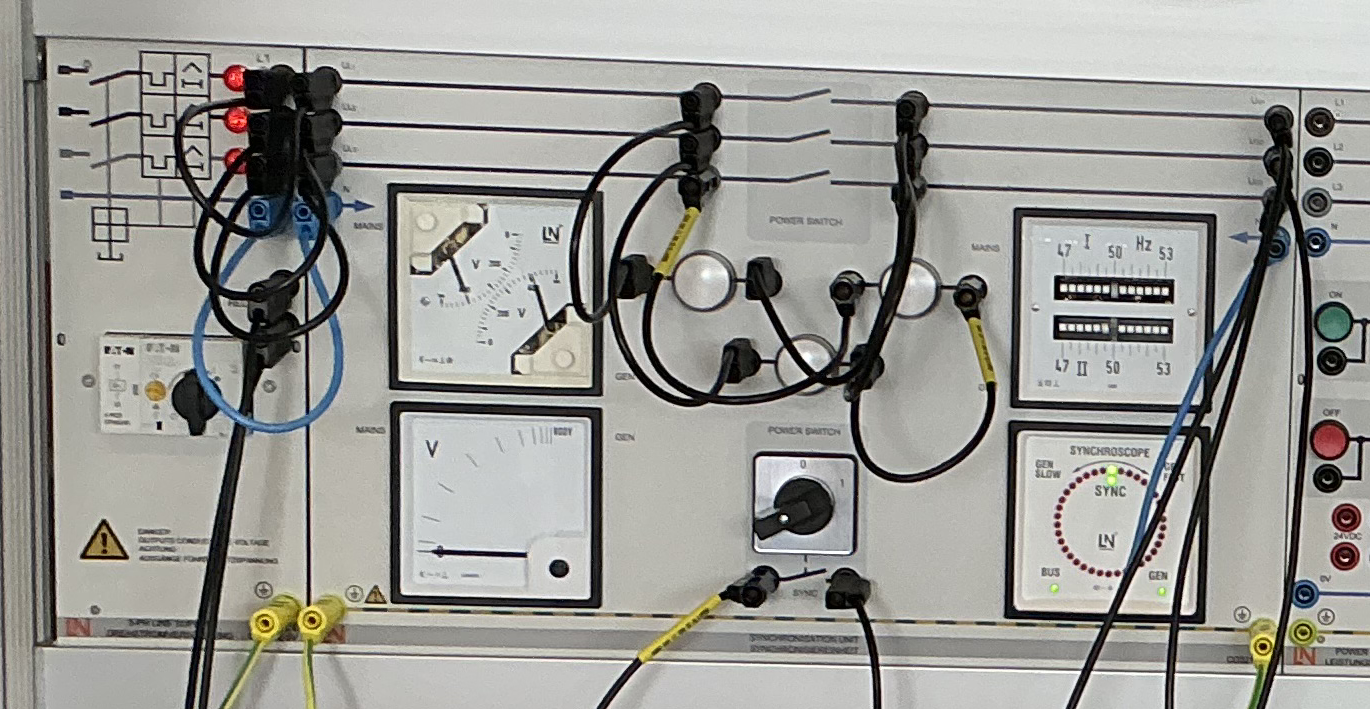
\includegraphics[\lw=.7]{media/E1S1/picture3.png}
    \caption{Meter close up}
    \label{fig:meter}
\end{figure}

The experiment demonstrated that synchronisation can be achieved reliably using the dark
lamp method. Furthermore, the experiment illustrated the importance of matching voltage,
frequency and phase angle before connecting a synchronous generator to the electrical
grid.

\subsection{Automatic Grid Synchronization}
Following the manual synchronization phase, the experiment transitioned to an
automated grid-coupling procedure using the system's digital control. This method
utilizes a centralized control unit to automatically monitor, adjust, and couple the
synchronous generator to the electrical grid, eliminating human error and timing
mistakes.

\subsubsection{Synchronization with the Multifunctional Relay}
The initial phase required a reconfiguration of the circuit in a way to shift control from
the manual to the automated system. The team disconnected the manual wiring
components, as the dark lamp circuit and manual synchronoscope were no longer
required for this procedure. The circuit was modified to focus entirely on interfacing the
machine with the automatic synchronization unit and the Multifunctional relay
(CO3301-5W).
\begin{figure}[H]
    \centering
    
\includegraphics[\lw=.7]{media/E1S2a/picture3.png}
    \caption{Final setup for synchronisation with Multifunctional relay}
\end{figure}
The machine setup was configured into "Sync mode" via the control software
touchscreen.
\begin{figure}[H]
    \centering
    
\includegraphics[\lw=.45]{media/E1S2a/picture1.png}
    \caption{Setting the Sync Mode in the Servo machine test system}
\end{figure}

The initial baseline voltage for the system was set to 45 V. Following the step-by-step
procedures outlined in the Laboratory Instructions for synchronous generator, the
target control parameters were programmed into the user interface. Once a secure
connection to the multifunctional relay unit was established, a software delay of 90
seconds was initiated to allow the system parameters to stabilize before execution.
The team did not encounter issues with the time-out monitoring; increasing the delay
to 120 s was therefore not needed.

\begin{table}[ht!]
    \centering
    \caption{Table of the delay parameter from Labsoft}
    \begin{tabularx}{.75\textwidth}{XXX}
        \toprule
        \textbf{ID} & \textbf{Name} & \textbf{Parameter}\\
        \midrule
        3063 & Time-out & 90 s (default: 60 s)\\
        \bottomrule
    \end{tabularx}
\end{table}

\subsubsection{Automatic Synchronization Execution}
Once the parameters were set and the "Run" command was executed, the integrated
WOODWARD easygen-2500 control system took full autonomous control over the
system. After starting it, the uncoupled generator was running at a standalone
rotational speed of 1420 rpm and an un-synchronized frequency of 47 Hz.
\begin{figure}[H]
    \centering
    \includegraphics[\lw=.8]{media/E1S2b/picture2.png}
    \caption{Setting the generator's parameters}
\end{figure}

Recognizing that the generator frequency was below the rigid 50 Hz grid standard, the
WOODWARD easygen-2500 controller automatically began increasing the prime
mover's RPM to bring the two systems into alignment. The automated control unit
continuously modulated the system, driving the generator through a ramp-up
sequence; the rotational speed was automatically accelerated from 1470 rpm up to the
exact synchronous speed of 1500 rpm. The internal generator frequency was adjusted
from 47 Hz up to the matching grid frequency of 50 Hz. The terminal voltage was
regulated upwards from the initial 45 V to a synchronized 48 V, drawing a measured
current of 0.61 A.

The control unit monitored the relative phase angle between the generator and the
network. The exact instant all synchronization conditions such as equal voltage
magnitude, frequency, and phase angle were achieved, the relay closed the internal
contacts. This successful coupling was confirmed by an audible physical "click" from
the power switch module, and the software interface instantly updated the system
status to all green lights.

\begin{figure}[H]
    \centering
    
\includegraphics[\lw=.75]{media/E1S2b/picture1.png}
    \caption{Grid Overview showing that the generator is connected}
\end{figure}
\newpage

\subsection{Automatic active power control}
\subsubsection{Theory}
A generator in island mode is feeding its own power system and delivers a frequency that
depends on the speed it rotates. The speed then depends on the mechanical torque and the
loads connected. For a constant speed the drive and load torque must be equal
(steady state). 

So, when the generator is connected to a three-phase grid, the speed it must rotate is
determined by the grid’s frequency. Before the generator can be connected, it must be
synchronised in terms of terminal voltage under no-load condition in magnitude,
frequency, phase sequence, and phase angle. 

In grid-parallel mode, since the grid dictates the rotation speed, the active power
output can only be adjusted by varying the drive torque at the generator shaft.
Increasing the drive torque via the speed controller does not increase the actual speed
but instead causes the rotor displacement angle to lead further in the direction of
rotation. This shift in the rotor angle relative to the grid voltage is what facilitates
the boost in active power output. 

A machine with non-salient pole or drum-type rotors operating at constant excitation
current and steady state can fall out of sync if a rotor displacement angle of 90$^\circ$
is exceeded. To prevent this from happening, a generator needs a power controller. The
controller will automatically correct the setpoint value specified for the output power. 

To manage the exchange of reactive power with the grid, the generator’s excitation
current must be controlled. An over-excited generator supplies lagging reactive power
(acting like a capacitor) and an under-excited generator consumes lagging reactive
power from the grid. By utilizing a $\cos\Phi$ controller within the multifunction relay, the
excitation voltage is automatically adjusted to maintain the desired power factor. 

In this part of the experiment, the $\cos\Phi$ controller of the multifunction relay is
tested to see how it works. The controller compares the generator’s power factor with a
setpoint value and provides feedback control pulses to the excitation voltage actuator.
This way a generator can run at a desired $\cos\Phi$ level. 

\subsubsection{Conducting the experiment}
Before the experiment is started, the parameters are checked as shown in \autoref{fig:setpoint}.
The 5520 initial load control setpoint 1 is set to 200 [kW]. The generator is then
connected to the three-phase grid using the multifunction relay. The experiment is to
change the setpoint value from 200 [kW] to 300 [kW] and then 400 [kW] and observe how
the output of apparent (S), active (P) and reactive power (Q) is.

\begin{figure}[H]
    \centering
    
\includegraphics[\lw=.85]{media/E1S2c/picture3.png}
    \caption{Software control of setpoint values}
    \label{fig:setpoint}
\end{figure}

After the setpoint is changed, a wait time is added until the system has settled into
steady state. Then the values are collected from the controller (\autoref{fig:PAC}) and
put into \autoref{tab:power}. The software then plots the measurements as seen in
\autoref{fig:graph}.

\begin{minipage}[t]{.415\textwidth}
    \begin{figure}[H]
        \centering
        
\includegraphics[\lw]{media/E1S2c/picture1.png}
        \caption{$\cos\Phi$ controller}
        \label{fig:PAC}
    \end{figure}
\end{minipage}
\hfill
\begin{minipage}[t]{.6\textwidth}
    \begin{figure}[H]
        \centering
        \includegraphics[\lw]{media/E1S2c/picture2.png}
        \caption{Graph setpoint and measured values}
        \label{fig:graph}
    \end{figure}
\end{minipage}

\begin{table}[ht!]
    \centering
    \caption{Measured values S, P, Q of setpoints}
    \label{tab:power}
    \begin{tabular}{lccc}
        \toprule
        \textbf{P set (kW)} & \textbf{200} & \textbf{300} & \textbf{400}\\
        \midrule
        S HMI (VA) & 196 & 310 & 445\\
        P HMI (W) & -193 & -292 & -390\\
        Q HMI (Var) & 35 & 99 & 207\\
        \bottomrule
    \end{tabular}
\end{table}

\subsubsection{Results and conclusion}
The graph in \autoref{fig:graph} shows the relation of setpoint power P [kW] to the
measured values of active (P HMI [W]) and reactive (Q HMI [Var]) power. As the setpoint
is increased from 200 to 400 [kW], the magnitude of the active power increases from 193
to 390 [W]. Simultaneously, the reactive power increases from 35 to 207 [Var].

This result shows that the active power controller successfully responds to the setpoint
changes. The simultaneous rise in reactive power suggests that the system maintains a
specific $\cos\Phi$, because more active power is transferred, the excitation is adjusted
to provide the necessary lagging reactive power to the grid in grid-parallel operation. 

\newpage

\section{Pumped-storage power stations}
A pumped-storage power plant uses electricity to pump water from a lower-level
reservoir to an upper-level reservoir where extra electricity production capacity is
available. Water flowing back down from the upper reservoir to the lower one powers
the synchronous machine acting as a generator. The test system replaces hydraulics with
an electrical motor-generator unit, a multifunction relay, and the SCADA.

The active and reactive power compensation experiment was not conducted; hence, only the
theoretical concept of its operation is analyzed.

\subsection{Power regulation}
The conducted experiment involved semi-automatic changes. In such an operating
mode, the automatic controls start up and synchronize the machine, and the operator specifies the
required values of active/reactive power in the SCADA.

\subsubsection{Theory}
In grid-parallel mode, the speed of the machine is determined by the grid frequency.
For a four-pole machine operating at a frequency of 50 Hz, the synchronous
speed will be around 1500 rpm.

The reactive power is controlled using excitation. If the excitation is increased,
the machine is over-excited and supplies reactive power to the grid. If the excitation
is decreased, the machine is under-excited and absorbs reactive power from the
grid.
\begin{figure}[H]
    \centering
    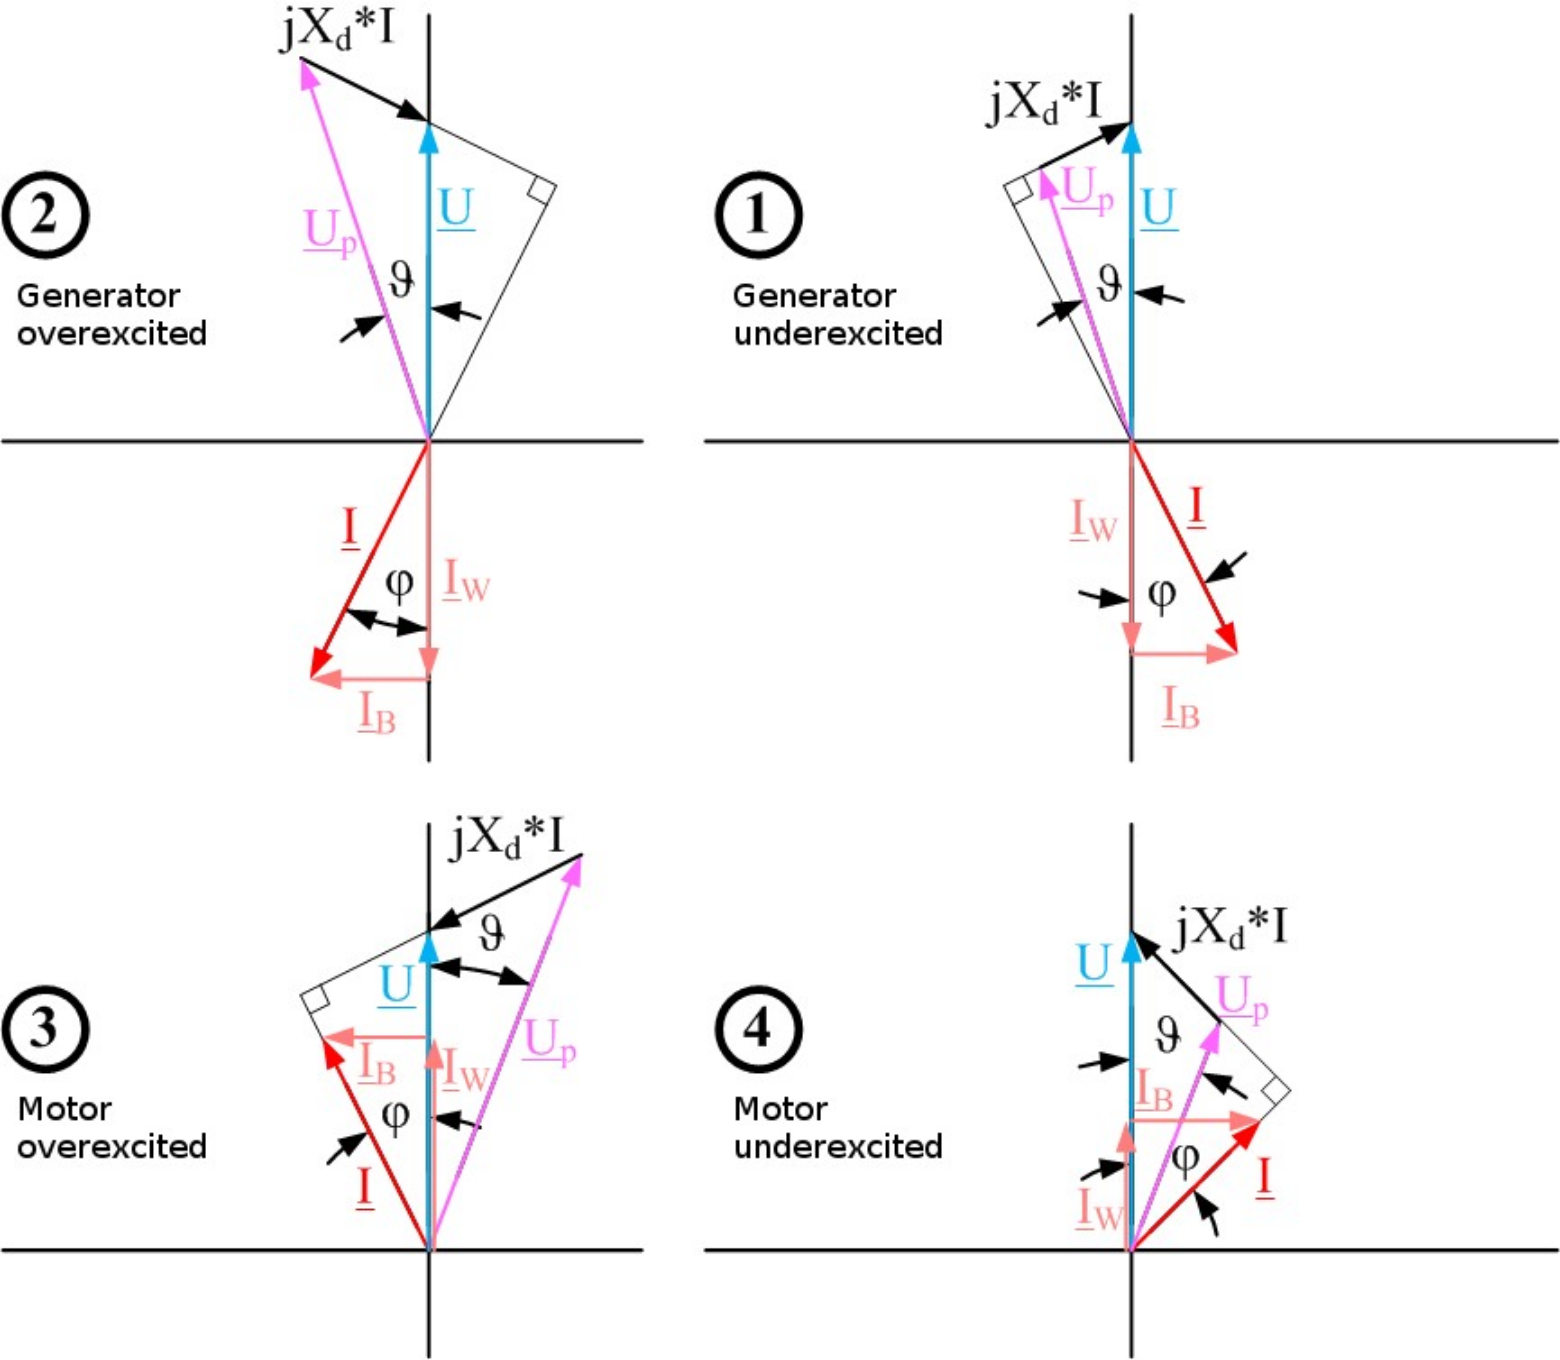
\includegraphics[\lw=.65]{media/E2S1a/reactive-power.png}
    \caption{Voltages and currents of a synchronous machine during four-quadrant operation}
    \label{fig:reactivepower}
\end{figure}

The active and reactive power sliders then define $P$ and $Q$ as percentages of this
apparent power limit:
\[
    P_\text{set} = \frac{P_{\%}}{100} \, S_\text{max},
    \qquad
    Q_\text{set} = \frac{Q_{\%}}{100} \, S_\text{max}.
\]

\subsubsection{Experimental setup}
This experiment involved the following equipment: pumped-storage training system,
synchronous machine, test bench for servo machine, excitation voltage controller,
multifunction relay, power supply, measuring units, and SCADA Viewer.

The connection of the machine to the network was carried out using the multifunction
relay, which performed the automatic synchronization and protection operations.
\begin{figure}[H]
    \centering
    
\includegraphics[\lw=.8]{media/E2S1a/picture3.png}
    \caption{Pumped-storage laboratory setup}
    \label{fig:eug3-setup-before}
\end{figure}

The voltage excitation was initially switched off. The multifunction relay was put
into AUTO mode, and then using the SCADA interface, the machine was started, and the
power was referenced. In the semi-automatic testing process, the load following feature
remained disabled, thus allowing the active and reactive power to be manually controlled
through the SCADA sliders.

\subsubsection{Procedure}
The experiment was conducted as follows:
\begin{enumerate}
    \item Parameter file named \texttt{EUG3\_400V\_50Hz.pvc} was loaded on the SCADA
    viewer.
    \item The servo-machine test stand, three-phase power supply, and excitation system were
    arranged as per lab guidelines.
    \item Multi-function relay was set to AUTO mode.
    \item SCADA diagnostics were initialized, and the synchronous machine was operated by
    STARTUP command.
    \item As soon as the generator circuit breaker was closed, LOAD FOLLOWING was not turned
    ON.
    \item The limit of apparent power and active/reactive power references were imposed
    through SCADA sliders manually.
    \item Machine speed, torque, voltage, active/reactive power, and power factor were
    measured by SCADA interface and attached sensors.
    \item The experiment was ended using the SCADA shutdown procedure.
\end{enumerate}

\subsubsection{Results}
\autoref{fig:eug3-scada} presents the SCADA display during the semi-automatic
power regulation test. The multi-function relay was active, and the machine was in RUN
mode. The motor-generator system was running at roughly synchronous speed.

\begin{figure}[H]
    \centering
    
\includegraphics[\lw=.85]{media/E2S1a/picture1.png}
    \caption{SCADA interface during semi-automatic power regulation}
    \label{fig:eug3-scada}
\end{figure}

The main measured values in SCADA are summarised in \autoref{tab:eug3-results},
with the Manual Control values of\\
$P_\text{set} = 70\%\ S_\text{max} \approx 560$ [W] and $Q_\text{set} = 0\%\ S_\text{max} = 0$ [Var].

\begin{table}[H]
    \centering
    \caption{Observed operating values during semi-automatic power regulation}
    \label{tab:eug3-results}
    \begin{tabular}{lcc}
        \toprule
        \textbf{Quantity} & \textbf{Measured value} & \textbf{Unit}\\
        \midrule
        Operating state & \makecell{RUN --\\Presetting} & -- \\
        Machine speed & 1499 & rpm \\
        Torque & -3.39 & Nm \\
        Grid line-to-line voltage & 411 & V \\
        Generator line-to-line voltage & 412 & V \\
        Generator apparent power $S$ & 429 & VA \\
        Generator active power $P$ & -427 & W \\
        Generator reactive power $Q$ & 14 & Var \\
        Power factor $\cos\Phi$ & 1.00 & -- \\
        Stored energy display & 97 & Wh \\
        \bottomrule
    \end{tabular}
\end{table}

Moreover, the local test stand machine also exhibited a speed near 1500 rpm, implying
that the machine had been synchronized with the frequency of the grid network. The
torque variation proved that the active power reference was implemented mechanically
rather than through speed alteration.

\subsubsection{Analysis and conclusion}
The results of the experiments were consistent with the expected behaviour of a
grid-connected synchronous machine. Once synchronised, the speed of the machine remained
constant, equal to the synchronous speed determined by the 50 Hz frequency of the grid.
Therefore, an increase in active power was achieved not by changing the speed, but rather
by changing the load angle and torque.

The value of reactive power was quite small in comparison with the value of active
power and the power factor was very close to 1.00. Thus, excitation was regulated in such
a way that very little reactive power was transferred back to the grid. The small non-zero
value of $Q$ may be due to some losses in the machine and the tolerance of the controller,
as well as the fact that measurements were made while the system had not yet settled
onto a steady state.

Semi-automatic start-up is a procedure where the user specifies the power references
manually, while the PLC and multifunction relay conduct all other actions to complete
the process of start-up. In contrast to fully automatic procedures, here the operator
must press a button to turn on the generator.

The semi-automatic pumped-storage experiment showed how a synchronous motor-generator set
can be started, synchronised and power-controlled through a SCADA interface.
The observed active power was controlled through torque, while the reactive power
remained close to zero due to excitation control.

\subsection{Active and reactive power compensation}
During the active-reactive power compensation test experiment, the LOAD FOLLOWING feature
of SCADA will be used. In this case, the system computes the values of active and
reactive power at the balance node and controls the motor-generator to provide compensation
for the externally added load. The active power compensation applies only to a resistive
load while both active and reactive power compensations apply to the inductive load.
This is done with the objective of minimizing the value of net power flow at the balance
node to near zero within the limits of current, reactive power and the apparent power
available in the machine.

The above-mentioned compensation was not done during the laboratory experiments.
The anticipated behavior should be that once the load switch is closed, the system adjusts
the output of the motor-generator upward or downward until the $\sum P$ and $\sum Q$
values at the balance node are minimized. Active power compensation is achieved by
changing the torque and therefore the active power output of the motor-generator set.
Reactive power compensation is achieved by changing the excitation of the synchronous
machine.

\newpage
\appendix
\section{Appendix}

\listoffigures

\listoftables

\printbibliography

\section*{Declarations on the use of AI tools}
``\textit{ChatGPT 5.5}'' was used to enhance vocabulary.\\
{\color{darkgray!95}{\textit{All sentences originate from our own ideas and were refined with the support of this tool.}}}\\
\url{https://chatgpt.com/}
\thispagestyle{fancy}
\end{document}
